\section{Extension of the model element}

In order to encode the structures needed to define and use multistate and multi-component complexes, the element \class{model} is extended to be linked to a list of \class{SpeciesType}s and a list of \class{Selector}s.

\begin{figure}[H]
\begin{center}
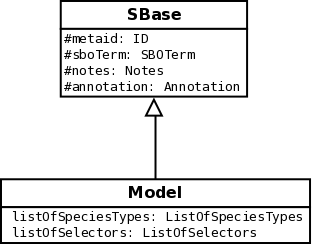
\includegraphics[scale=0.3]{figs/pngs/ModelClass.png} 
\caption{Definition of \class{Model} and its relation with \class{SBase}.}
\label{fig:Model}
\end{center}
\end{figure}

\begin{example}
<model xmlns:multi="http://www.sbml.org/sbml/level3/version1/multi/version1">
  <!-- some compartments -->
  <multi:listOfSpeciesTypes>
    <!-- some species types -->
  </multi:listOfSpeciesTypes>
  <multi:listOfSelectors>
    <!-- some selectors -->
  </multi:listOfSelectors>
  <!-- some species, initialAssignments, rules,  reactions, events -->
</model>
\end{example}